\documentclass[DIV=calc,paper=a4,fontsize=11pt,twocolumn]{scrartcl}

\usepackage{lipsum}
\usepackage[english]{babel}
\usepackage{fourier}
\usepackage[protrusion=true,expansion=true]{microtype}
\usepackage{amsmath,amsfonts,amsthm}
\usepackage[svgnames]{xcolor}
\usepackage[hang,small,labelfont=bf,up,textfont=it,up]{caption}
\usepackage{booktabs}
\usepackage{fix-cm}
\usepackage{graphicx}
\usepackage{url}

\usepackage{sectsty}
\allsectionsfont{\usefont{OT1}{phv}{b}{n}}

\usepackage{fancyhdr}
\pagestyle{fancy}
\usepackage{lastpage}

% Headers - all currently empty
\lhead{}
\chead{}
\rhead{}

% Footers
\lfoot{}
\cfoot{}
\rfoot{\footnotesize Page \thepage\ of \pageref{LastPage}}

\renewcommand{\headrulewidth}{0.0pt} % No header rule
\renewcommand{\footrulewidth}{0.0pt} % Thin footer rule

\usepackage{titling}

\newcommand{\HorRule}{\color{DarkGrey}\rule{\linewidth}{2pt}}

\pretitle{\vspace{-50pt}
  \begin{flushleft}
    \HorRule
    \fontsize{30}{30}
    \usefont{OT1}{phv}{b}{n}
    \color{SteelBlue}
    \selectfont}

\title{Patient data storage security}

\posttitle{\end{flushleft}\vspace{-10pt}}

\preauthor{\begin{flushleft}\large
    \usefont{OT1}{phv}{b}{n}
    \color{SteelBlue}}

\author{Optinomic GmbH}

\postauthor{\end{flushleft}\vspace{-20pt}}

\predate{\begin{flushleft}
    \usefont{OT1}{phv}{b}{n}
    \color{SteelBlue}}

\date{12 October 2013}

\postdate{\end{flushleft}\vspace{-10pt}\HorRule}

\begin{document}

\maketitle

\thispagestyle{fancy}

{\setlength\parindent{0pt} \textbf{The prevalence of mHealth
    applications is increasing rapidly in the European market.  The
    measurement of therapy-relevant patient parameters and the
    delivery of therapeutic advice via patients' own mobile devices
    (smartphones and tablets) poses new challenges in the area of data
    protection.  In this paper we present a proposed plan for patient
    data management in the Optinomic survey and cognitive testing
    management framework.  This plan is intended to provide strong
    data protection guarantees while maintaining flexibility and
    usability for patients and therapists.  A cryptographically secure
    mechanism is used to ensure that patient survey responses can be
    collected from a patient's own mobile device, but can then only be
    associated with patient identifying information within the context
    of a secure server maintained behind a clinic firewall.}}

\section*{Data storage for mHealth}

There is good evidence that monitoring of patient mental states and
delivery of therapeutic material to patients outside of a clinical
setting can lead to improved therapeutic outcomes.  The ubiquitous use
of mobile devices such as smartphones and tablets provides a clear
opportunity to provide such ``extra-clinical'' support to patients,
and modern web application technology permits the development of
frameworks that can help therapists to manage the information
collected from their patients and to monitor patient states to aid in
early intervention in potential problems.

Optinomic is developing a framework to provide adaptive monitoring of
patient states, treatment compliance and therapeutic outcomes via
surveys and simple cognitive tests delivered to smartphones, tablets
or patients' desktop computers.  The Optinomic system will integrate
with existing Clinical Information Systems, will aid in the collection
of legally mandated patient information (e.g. the intake surveys
required for the treatment of substance abuse disorders), and will use
modern statistical methods to enable therapists and researchers to
model patient progress more effectively.

Collection of data using mobile devices and internet technologies has
serious implications for compliance with data protection regulations.
Patient data is no longer rigidly confined within a clinic's
information technology systems where it can be monitored and
controlled.  This means that careful analysis is needed to ensure that
whatever methods are used to collect patient data provide strong data
protection guarantees.


\section*{Security implications}

Within the framework of the applications that we propose, there are
two classes of information that must be considered.  First, there is
\emph{patient identifying information}: patient names, unique
identifiers used within Clinic Information Systems, gender, date of
birth, treatment history, email addresses, and so on.  This
information must be protected and should not be accessible to any
entities outside of a clinic's security firewall.

The second class of data comprises patient responses to surveys and
results of cognitive tests.  This data has no \emph{intrinsic}
confidentiality requirements -- its confidentiality requirements arise
solely from the possibility of associating such data with the patient
from whom it originated.  There should be no way to connect patient
survey responses to patient identifying information \emph{except}
within the setting of an approved system within the clinic firewall.

The core problem is thus that we would like for patients to be able to
access Optinomic applications from their own mobile devices and home
computers using the browser that they are familiar with, without
needing to take any special security precautions themselves, while at
the same time guaranteeing a secure separation between patient
identifying information and patient survey responses.


\section*{Proposed solution}

The architecture that we propose is as follows:

\begin{itemize}
  \item{We use a private \emph{therapy management server} lying within
    the clinic security firewall along with a publicly accessible
    \emph{survey server}.  The therapy management server, being within
    the clinic firewall, will be managed according to the security and
    data protection policies of the clinic.}
  \item{All scheduling of patient survey and test activities is done
    by the therapy management server.}
  \item{The \emph{only} link between a patient and his/her survey/test
    activity is a randomly generated \emph{survey ticket}.}
  \item{There is no correlation between survey tickets for the same
    patient, or between survey tickets for the same survey or test
    module, and there is no temporal correlation of tickets,
    preventing correlation attacks based on ticket allocation.}
\end{itemize}

The operation of this architecture is best illustrated with a detailed
view of the primary use case: the scheduling, execution and collection
of data for a single activation of a survey module for a single
patient.


\section*{Use cases}

The primary use case we will present here is for a therapist
scheduling a patient survey activity and the subsequent presentation
of the survey to the patient, followed by data collection.  This use
case highlights most of the pertinent issues surrounding patient data
security for our applications.  Some further use cases are considered
below.

\subsection*{Primary use case}

\begin{figure*}
  \begin{center}
    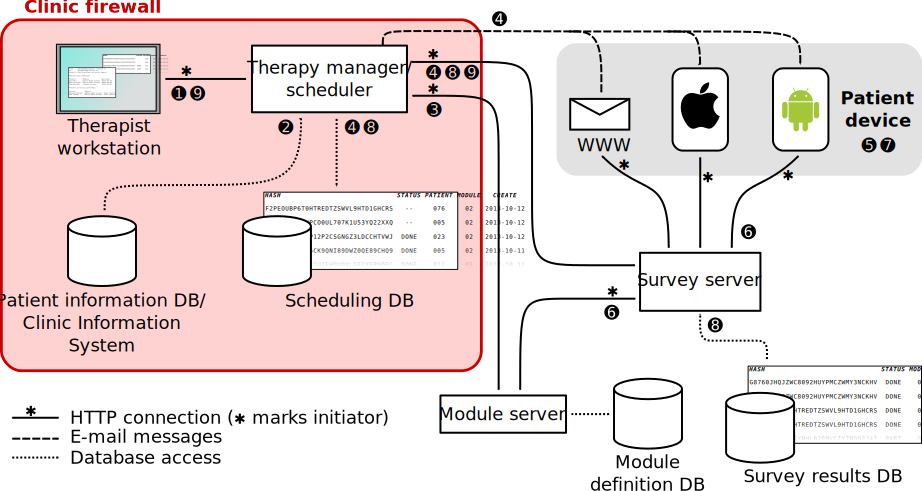
\includegraphics[width=\textwidth]{flow-diagram-en}
  \end{center}
  \caption{Data flow diagram for primary survey scheduling use case.
    See text for step-by-step explanation.}
  \label{fig:flow-diagram}
\end{figure*}

The numbering of the following steps corresponds to the numbered
interactions displayed in Figure~\ref{fig:flow-diagram}:

\begin{enumerate}
  \item{The therapist interacts with the Optinomic system from a
    workstation lying within the clinic's existing IT firewall, where
    it can be managed in accordance with the data protection policies
    of the clinic.  The therapist uses a web browser to connect to the
    Optinomic therapy management server which also lies within the
    clinic firewall.  Because both the therapist workstation and the
    therapy management server lie within the clinic firewall, this
    connection can be made using a normal HTTP connection.  If the IT
    policies of the clinic permit therapists to access clinic systems
    from outside the clinic firewall using VPN or other secure
    connections, this path is also an option for connecting to the
    Optinomic server.}
  \item{The therapist is then able to access patient details, using
    either a link to an existing Clinic Information System or an
    Optinomic patient details DB.  All of these components are
    contained within the clinic firewall, so there is no possibility
    of compromise of patient details.}
  \item{The therapist selects a therapeutic module (survey or
    cognitive test) to schedule for a patient by browsing through
    module definitions stored on a module server (the \emph{Module
      Market}).  No patient data is associated with these module
    definitions and the module server can thus lie outside the clinic
    firewall (in many cases, we would recommend that module
    definitions be accessed from a central Optinomic server so that
    the latest module versions are always available).  Access to the
    module server is initiated by the therapy management server and
    uses a normal HTTP connection.}
  \item{The critical step in the data flow is the scheduling of the
    module for a patient.  There needs to be an association made
    between a unique patient identifier and an instance of the
    activation of the module.  The patient also needs to be informed
    that the module is available to work on.  In order to permit the
    patient to use their own mobile devices to complete surveys
    without compromising patient identifying information (name, unique
    patient ID, email address, and so on) to servers outside the
    clinic firewall, a random \emph{survey ticket} is generated.  This
    survey ticket is a 32-character string of letters and digits that
    is generated by the therapy management server for each module
    activation.  The only place where a link is made between this
    random string and the patient ID is an entry created in the
    Optinomic scheduling database which lies within the clinic
    firewall and is accessed only by the therapy management server.
    Once the scheduling database entry has been created, the survey
    ticket and details of the module to be activated are passed to the
    \emph{survey server}.  Note that no patient identifying
    information is passed to the survey server, which runs on a
    machine outside the clinic firewall and can be accessed directly
    by patients from their own mobile devices or desktop computers.
    All processing on the survey server is done in reference to these
    randomly generated survey tickets.  Once the survey server has
    been notified of the module activation, the therapy management
    server sends an email to the patient's registered email address
    notifying the patient that a new module activation is available
    (note again that patient email information is \emph{not} sent to
    the survey server).}
  \item{At some point later in time, the patient accesses their email,
    using whatever mobile device or email client that they normally
    use and they see that they have a message from the Optinomic
    therapy manager.  This message contains a URL pointing to the
    relevant survey page, based on the survey ticket generated by the
    therapy manager
    (e.g. \url{http://www.optinomic.ch/G8760JHQJZWC8092HUYPMCZWMY3NCKHV}).}
  \item{When the patient follows the URL in the email message, the
    survey server generates HTML pages and Javascript code to run the
    relevant survey or cognitive test on the patient's mobile device
    or computer.  Because the survey contents is accessed only via the
    random survey ticket, this connection can be made via a normal
    HTTP connection.}
  \item{The patient completes the survey on their mobile device.  When
    they are done, the survey results are submitted to the survey
    server.}
  \item{When the survey server receives the results from a survey, it
    saves them to a survey results database.  This database is keyed
    by the random survey ticket, so there is no means by which survey
    results can be associated with patient identities\footnote{The
      only exception to this statement is (obviously) if the module
      directly requests patient identifying information as part of a
      survey.}.  Once the survey results are saved, the survey server
    sends a message to the therapy management server to indicate that
    the survey has been completed.  Note that this message is the
    \emph{only} instance where communication is required to cross the
    clinic firewall in an incoming direction.  As such, survey
    completion messages are transmitted from the survey server to the
    therapy management server using a custom channel over a single IP
    port opened in the clinic firewall, rather than via a normal HTTP
    connection.  When the therapy management server receives this
    message from the survey server, it updates the scheduling database
    to indicate that the patient has completed the assigned activity
    (at this point, the management server could also send alerts to
    the therapist, trigger follow-on activities for the patient, and
    so on).}
  \item{At some point later in time, the therapist once again connects
    to the therapy management server to view the survey results.  The
    therapy management server is able to access these results from the
    survey server using a normal HTTP connection.  Because the therapy
    management server has access both to the survey results database
    (via the survey server) and the scheduling database, it is able to
    associate survey results to patient identities using the link
    between the random survey tickets and patient identities stored in
    the scheduling database.}
\end{enumerate}


\subsection*{Other use cases}

There are a range of other use cases that are of interest in terms of
data security issues.  Here we mention three, to indicate how typical
uses of the Optinomic system are unlikely to result in compromise of
patient data confidentiality.

\paragraph{Survey interruption and resumption}

For longer surveys, it may be desirable for patients to be able to
interrupt and later resume survey completion.  There are two possible
approaches here: if we permit activities to be paused and resumed only
on the same device, then intermediate survey results can simply be
stored in a browser cookie for later access.  On the other hand, if a
patient wants to partially complete a survey on one device (a home
computer, perhaps) then finish the survey on another device (a
smartphone, for example), then partial survey results can be saved to
the survey server.  Neither of these approaches risks compromise of
the link between patient identity and survey results.

\paragraph{Patient monitoring}

The survey completion messages sent from the survey server to the
therapy management server allow for prompt notification of the
therapist of when patients complete certain activities.  Because all
scheduling and survey completion information is available in the
scheduling database, the therapy management server can easily generate
reports of patient activity for therapist monitoring, and can also
alert the therapist to any concerning patterns of patient
non-compliance.  All data processing that requires association of
survey results with patient identities occurs solely within the clinic
firewall, so there is no risk of compromise of patient
confidentiality.

\paragraph{Temporal change}

One of the major benefits of the type of extra-clinical patient
monitoring proposed by Optinomic is that it enables ongoing monitoring
of patient progress and emotional states.  Automated scheduling of the
collection of patient data via lightweight daily ``mini-surveys''
permits the accumulation of long time series of patient data.
Combined with simple data visualisation, this allows the therapist to
demonstrate therapeutic progress to patients in a very direct way: for
example, ``In the last month, your daily self-assessment mood scores
have been consistently higher than in any of the preceding three
months''.  Again, for any data analysis of this type, all data
processing requiring association of survey results with patient
identities occurs solely within the clinic firewall, so there is no
risk of compromise of patient confidentiality.


\section*{Conclusions}

The proposed split between the storage of patient identifying
information and survey/test results, using randomly generated survey
tickets to provide the link between the two types of data, is
guaranteed to protect against breaches in patient data
confidentiality.  There is no flow of patient identifying data out of
the clinic firewall and there is no possibility of making a link
between patient survey results and patient identities outside of the
firewall, since the only information associating patient identities
and survey tickets is stored in the Optinomic scheduling database
which is situated within the clinic firewall.

\end{document}
